\chapter{Best Response Sequences in the Iterated Prisoner's Dilemma}\label{chapter:best_response_sequence}

\begin{center}
    The research reported in this Chapter has been carried out with:

    Axelrod-Python library version: 4.2.0 \\
    Associated data set: \cite{Glynatsi2020_sequences} \\ \vspace{.5cm}
\end{center}

\hrulefill

\section{Introduction}

In this Chapter best response strategies are explored in the form
of static sequences of moves, in order to generate a large data set of best
response sequences to a collection of opponents.

The data set is generated by considering best response sequences in finite IPD
matches of 205 turns against \numberofstrategiesbestsequences strategies
available in the APL. These best response sequences are not obtained explicitly
but instead are estimated heuristically using a genetic algorithm devised for
this purpose.

The purpose of a large collection of best response sequences is
to serve as training data in Chapter~\ref{chapter:lstm} which aims to train a
recurrent neural network as an IPD strategy. In Chapter~\ref{chapter:lstm} the
usage of the bespoke data set, which has been archived and made publicly
available~\cite{Glynatsi2020_sequences}, is discussed in more details. This
Chapter is structured as follow:

\begin{itemize}
    \item section~\ref{section:ipd_as_sequences} formalises the use of sequences to express a player in a
    finite IPD match.
    \item section~\ref{section:genetic_algorithm} describes the genetic algorithm
    used to estimate best response
    sequences.
    \item section~\ref{section:generating_sequences} details the process of
    generating best response sequences to a collection of
    \numberofstrategiesbestsequences strategies.
\end{itemize}

\section{Iterated Prisoner Dilemma Strategies as Sequences}\label{section:ipd_as_sequences}

In a finite \(N\) round IPD match a player that does not react to their opponent
can be defined by a sequence,

\begin{equation}
    S \in \{C, D\} ^ n, \text{where } 1 \leq n \leq N.
\end{equation}

Strategies that base their actions on sequences are already established in the
literature~\cite{Beaufils1997}, such as Periodic Player \(CD\), Periodic Player \(DC\),
Periodic Player \(CCD\) and Periodic Player \(DDC\)~\cite{Li2011, Mittal2009},
or as referred to in~\cite{Knight2016} Cycler \(CD\), Cycler \(DC\),
Cycler \(CCD\) and Cycler \(DDC\). These are strategies that play a given sequences
periodically, however, the strategies concerned with here play a given
sequence only once, thus \(n = N\).

As an example consider a match of 10 turns between the strategy \(S = \{D, D, D,
C, C, C, D, D, C, C\}\) and Cooperator. The match between the two strategies
is captured by Table~\ref{table:s_vs_cooperator} where \(U(s_1, s_2)\in
\mathbb{R}^2\) is the average score per turn scored by strategies \(s_1\) and
\(s_2\).

\begin{table}[htb]
\centering
\begin{tabular}{cccccccccccc}
    & \textbf{1} & \textbf{2} & \textbf{3} & \textbf{4}  & \textbf{5} & \textbf{6} & \textbf{7} & \textbf{8}  & \textbf{9} & \textbf{10} & 
    \(U(S, \text{Cooperator})\) \\ \midrule
    \(S\) & \(D\) & \(D\) & \(D\) & \(C\) & \(C\) & \(C\) & \(D\) & \(D\) & \(C\) & \(C\) & 4.0 \\
    Cooperator & \(C\) & \(C\) & \(C\) & \(C\) & \(C\) & \(C\) & \(C\) & \(C\) & \(C\) & \(C\) & 1.5 \\ \bottomrule
\end{tabular}
\caption{The interactions of a 10 turns match between \(S = \{D, D, D, C, C, C, D, D, C, C\}\) and
Cooperator as well as the average score per turn achieved by each strategy.}\label{table:s_vs_cooperator}
\end{table}

A sequence strategy \(S\) can play against strategies that react to the history,
for example against Tit Tor Tat as demonstrated by Table~\ref{table:s_vs_tft},

\begin{table}[htb]
\centering
\begin{tabular}{cccccccccccc}
    & \textbf{1} & \textbf{2} & \textbf{3} & \textbf{4}  & \textbf{5} & \textbf{6} & \textbf{7} & \textbf{8}  & \textbf{9} & \textbf{10} &
    \(U(S, \text{Tit For Tat})\) \\ \midrule
    \(S\) & \(D\) & \(D\) & \(D\) & \(C\) & \(C\) & \(C\) & \(D\) & \(D\) & \(C\) & \(C\) & 2.2 \\
    Tit For Tat & \(C\) & \(D\) & \(D\) & \(D\) & \(C\) & \(C\) & \(C\) & \(D\) & \(D\) & \(C\) & 2.2 \\ \bottomrule
\end{tabular}
\caption{The interactions and average score per turn of a 10 turns match between
\(S = \{D, D, D, C, C, C, D, D, C, C\}\) and Tit For Tat.}\label{table:s_vs_tft}
\end{table}

and against stochastic strategies such as Random. Random cooperates with a
probability of \(0.5\) at each turn, and thus the actions of the strategy are
not deterministic. Random is a strategy that does react to the history, however,
the actions of stochastic strategies that react to the
history also differ between repetitions even when the history of the match is
the same. Tables~\ref{table:s_vs_random} and~\ref{table:s_vs_random_2} both
capture a match between \(S\) and a Random player. For a match of 10 turns
Random has a total of \(2^{10}\) possible plays.
In order to capture several different plays of stochastic strategies computer
seeding, further details of this are given in section~\ref{section:generating_sequences}.

\begin{table}[htb]
\centering
\begin{tabular}{cccccccccccc}
    & \textbf{1} & \textbf{2} & \textbf{3} & \textbf{4}  & \textbf{5} & \textbf{6} & \textbf{7} & \textbf{8}  & \textbf{9} & \textbf{10} &
    \(U(S, \text{Random})\) \\ \midrule
    \(S\) & \(D\) & \(D\) & \(D\) & \(C\) & \(C\) & \(C\) & \(D\) & \(D\) & \(C\) & \(C\) & 2.2 \\
    Random & \(D\) & \(D\) & \(C\) & \(C\) & \(D\) & \(C\) & \(D\) & \(C\) & \(C\) & \(D\) & 2.2 \\ \bottomrule
\end{tabular}
\caption{The interactions and average score per turn of a 10 turns match between
\(S = \{D, D, D, C, C, C, D, D, C, C\}\) and Random.}\label{table:s_vs_random}
\end{table}

\begin{table}[htb]
\centering
\begin{tabular}{cccccccccccc}
    & \textbf{1} & \textbf{2} & \textbf{3} & \textbf{4}  & \textbf{5} & \textbf{6} & \textbf{7} & \textbf{8}  & \textbf{9} & \textbf{10} & \(U(S, \text{Random})\) \\ 
    \midrule 
    \(S\) & \(D\) & \(D\) & \(D\) & \(C\) & \(C\) & \(C\) & \(D\) & \(D\) & \(C\) & \(C\) & 2.4 \\
    Random & \(C\) & \(D\) & \(D\) & \(C\) & \(C\) & \(C\) & \(D\) & \(D\) & \(C\) & \(C\) & 1.9 \\ \bottomrule
\end{tabular}
\caption{The interactions and average score per turn of a 10 turns match between
\(S = \{D, D, D, C, C, C, D, D, C, C\}\) and Random. The actions make by Random
are different to that of Table~\ref{table:s_vs_random}.}\label{table:s_vs_random_2}
\end{table}

As discussed in Chapters~\ref{chapter:introduction} and~\ref{chapter:memory_one},
a best response strategy is a strategy that achieves that most favourable outcome.
Thus a best response sequence against a given opponent \(Q\) corresponds
to a sequence \(S^*\) for which the average score per turn is maximised,
as given in~(\ref{eq:best_response_sequence}).

\begin{equation}\label{eq:best_response_sequence}
    \begin{aligned}
    \max_{S^*}: & U(S^*, Q)
    \end{aligned}
\end{equation}

Identifying best responses to some opponents can be a trivial problem. The
optimal sequence against a Cooperator is in an all \(D\) sequence. In fact the
sequence \(\{\underbrace{D, \dots, D}_{N}\}\) is a best response
against any sequence player whose plays are independent of the history.
However,
for some strategies identifying best responses is a complex problem.

Additionally, there are strategies that have multiple best response sequences. For
instance the strategy Adaptive introduced in~\cite{Li2011}. Adaptive opens by
playing a sequence of \(\{\underbrace{C, \dots, C}_{6}\}\) followed by a
sequence of \(\{\underbrace{D, \dots, D}_{5}\}\). The strategy then proceeds to
play either \(C\) or \(D\) depending on which action had a higher total score
for the strategy (the total score is recalculated at each turn). A sequence
maximises its average score against Adaptive by locking the strategy into
unconditional cooperations following its opening 11 turns sequence while the sequence
defects. In order
for cooperation to be the most favourable action for Adaptive the strategy needs to achieve
two mutual cooperations at its opening sequence. That is because the score achieved
by cooperating \(2 \times 3 + 4 \times 0 = 6\) is greater than the
score achieved by defecting \(1 \times 5 = 5\).
Any sequence which incorporates two cooperations in the first 6 turns
and defects thereafter is a best response sequence to Adaptive. Thus, there
can be \(2^{6}\) best response sequences to the strategy, for example \(S_{1}^*\) and \(S_{2}^*\),

\[S_{1}^* = \{C, D, D, D, D, C, D, D, D, D, D, D, D, D, D\}\]

\[S_{2}^* = \{D, D, C, C, D, D, D, D, D, D, D, D, D, D, D\}\]

where \(U(S_{1}^*, \text{Adaptive}) = U(S_{2}^*, \text{Adaptive}) = 3.4\).

Due to identifying best response sequences to some opponents being a complex
problem, and moreover, multiple best response sequences existing for some
opponents the best response sequences are not manually identified. Instead a
genetic algorithm is used to estimate them. A background on genetic algorithms
as well as the details of the specific genetic algorithm devised for this Chapter
are presented in the following section.

\section{Genetic Algorithm}\label{section:genetic_algorithm}

A genetic algorithm (GA) is a heuristic inspired by the process of natural
selection that belongs to the larger class of evolutionary algorithms. As stated
in~\cite{Whitley1994} GAs encode a potential solution to a
specific problem on a simple chromosome-like data structure, and apply
recombination operators to these structures in such a way as to preserve
critical information. GAs are often viewed as function
optimisers, although the range of problems to which they have been
applied is quite broad~\cite{Hou1994, Jones1997, Yang1998}.

An implementation of a GA begins with a \textit{population} \(P\) of
potential solutions, a number of \textit{generations} \(G \in \N\) and a cut-off or
\textit{bottleneck} \(b < |P|\). At each generation the algorithm scores and potentially
removes each member of the population \(p_i \in P\). This is done by using a
mapping from a member of the population to an ordered set based on an evaluation
function \(f\), usually \(f(p_i) \to \R\), and by only keeping the top \(b\)
ranking members (or proportion of members) by score at the end of each
generation. The rest of the member are discarded. By keeping the top ranked
individuals critical information regarding the successful candidates is
preserved and the population rebuilds on it by using a series of
\textit{crossovers} and \textit{mutations}.

\begin{itemize}
    \item During a crossover 2 members of the population are selected, and a new
    member is created based on combination of their ``genes''. The 2 selected members
    are commonly referred to as parents.
    \item Mutation is a probabilistic change that occurs to an individual,
    Mutation is commonly associated with a probability, denoted as \(p_m\).
    \(p_m\) is the probability of a mutation happening, either to the individual
    or to each gene of the individual.
\end{itemize}

A diagrammatic representation of a generic GA is given in Figure~\ref{fig:ga_flow_diagram}.

\begin{figure}[!htbp]
    \centering
    \includestandalone[width=.77\textwidth]{src/chapters/06/tex/ga_flow_diagram}
    \caption{Generic flow diagram of a GA.}\label{fig:ga_flow_diagram}
\end{figure}

The purpose of a GA here is to estimate a best response sequence to
a given opponent \(Q\). Consequently, the members of the population correspond to
sequences,

\[S_i \in P \text{ where } |S_i| = N\]

and the evaluation function corresponds to the
average score per turn of a sequence against \(Q\),

\[U(S_i, Q) \to \R \text{ for } S_i \in P.\]

More specifically, the exact GA used in this Chapter is given
by Algorithm~\ref{algorithm:genetic_algorithm}.

\begin{algorithm}[!htbp]
    \SetAlgoLined
    \KwIn{\(Q, N, b, p_m, G, K\)}
    \KwOut{The populations at each generation and the members' scores}
     \Begin{
     create initial population (Algorithm~\ref{algorithm:initial_population}) of members \(S\), where \(|S| = N\) and \(|P| = K\)\\
     \While{\(g_{i} < G\)}{
        score each member based on \(U(S_i, Q)\) for \(S_i \in P\) \\
        sort population based on scores \\
        keep \(b\) top members \\
        \While{\(|P|\) \(< K\)}{
            select 2 random members \\
            use members to create new member through crossover\\
            \For{gene in new member}{
            mutate gene with probability \(p_m\)}
            add new member to population\\
            }
     }}
     \caption{GA for estimating best response sequences to a given opponent \(Q\).}\label{algorithm:genetic_algorithm}
\end{algorithm}

The initial population is created using Algorithm~\ref{algorithm:initial_population}.

\begin{algorithm}[!htbp]
    \SetAlgoLined
    \KwIn{\(K, N\)}
    \KwOut{A population of size \(K\).}

    \Begin{
    set of cuts $\gets$ \(K\) evenly spaced numbers over \([1, N]\) \\
    \For{\(c \in\) set of cuts}{
        first new member $\gets$  \(\{\underbrace{C, \dots, C}_{c}, \underbrace{D, \dots, D}_{N-c}\}\) \\
        second new member $\gets$ \(\{\underbrace{D, \dots, D}_{c}, \underbrace{C, \dots, C}_{N-c}\}\) \\
        add both members to population
    }
        }
 \caption{Create initial population of individuals \(S\)}\label{algorithm:initial_population}
\end{algorithm}

Using a starting population of random guesses is a generally common approach in
the GA literature~\cite{Hou1994}. However, there is efficiency in using non
random starting populations~\cite{Drezner2005, Osaba2014}.
As discussed in section~\ref{section:ipd_as_sequences} the best response sequence
to any strategy that does not react to the history is a Defector. Moreover,
the best response sequence to several strategies include sequences mainly dominated
by cooperation expect in the last turns. These are
sequences that have been incorporated in the initial population. More specifically,
Algorithm~\ref{algorithm:initial_population} consider all the possible combinations
of:

\[\bullet \{\underbrace{C, \dots, C}_{c}, \underbrace{D, \dots, D}_{N-c}\} \text{ for } c \in \text{evenly spaced numbers over } [1, N] \text{ and}\]
\[\bullet \{\underbrace{D, \dots, D}_{c}, \underbrace{C, \dots, C}_{N-c}\} \text{ for } c \in \text{evenly spaced numbers over } [1, N].\]

The GA of Algorithm~\ref{algorithm:genetic_algorithm} has been implemented in the programming language Python
and it has been organised into a open source package called
\mintinline{python}{sequence_sensei} available at. %TODO archive
The properties of creating an initial population, crossover and mutation have been
implemented as individual functions.
The implementation of Algorithm~\ref{algorithm:initial_population} in the package
is given by Figure~\ref{fig:get_initial_population}.

\begin{figure}[!htbp]
\begin{sourcepy}
import numpy as np
def get_initial_population(half_size_of_population, sequence_length):
    """
    Generates an initial population of sequences. Note that the length
    of the population which is being generated is 2 * half_size_of_population.
    """
    cuts = np.linspace(1, sequence_length, half_size_of_population, dtype=int)
    sequences = []
    for cut in cuts:
        sequences.append(
            [1 for _ in range(cut)] + [0 for _ in range(sequence_length - cut)]
        )
        sequences.append(
            [0 for _ in range(cut)] + [1 for _ in range(sequence_length - cut)]
        )

    return sequences
\end{sourcepy}
\caption{Source code for the function \mintinline{python}{get_initial_population}
implemented in \mintinline{python}{sequence_sensei} which is used to create an
initial population of a given size.}\label{fig:get_initial_population}
\end{figure}

Figure~\ref{fig:get_initial_population_example} gives an example of creating an
initial population using the package. Note that the sequences are of 0s and 1s
and not IPD actions. The APL project can map binary number to actions such that
\(0 \to D\) and \(1 \to C\). This is also demonstrated in
Figure~\ref{fig:get_initial_population_example}.

\begin{figure}[!htbp]
    \begin{usagepy}
>>> import sequence_sensei as ss
>>> import numpy as np

>>> initial_population = ss.get_initial_population(
...     half_size_of_population=5, sequence_length=8
... )
>>> np.matrix(initial_population)
matrix([[1, 0, 0, 0, 0, 0, 0, 0],
        [0, 1, 1, 1, 1, 1, 1, 1],
        [1, 1, 0, 0, 0, 0, 0, 0],
        [0, 0, 1, 1, 1, 1, 1, 1],
        [1, 1, 1, 1, 0, 0, 0, 0],
        [0, 0, 0, 0, 1, 1, 1, 1],
        [1, 1, 1, 1, 1, 1, 0, 0],
        [0, 0, 0, 0, 0, 0, 1, 1],
        [1, 1, 1, 1, 1, 1, 1, 1],
        [0, 0, 0, 0, 0, 0, 0, 0]])

>>> import axelrod as axl
>>> np.matrix([[axl.Action(gene) for gene in member] for member in initial_population])
matrix([[C, D, D, D, D, D, D, D],
        [D, C, C, C, C, C, C, C],
        [C, C, D, D, D, D, D, D],
        [D, D, C, C, C, C, C, C],
        [C, C, C, C, D, D, D, D],
        [D, D, D, D, C, C, C, C],
        [C, C, C, C, C, C, D, D],
        [D, D, D, D, D, D, C, C],
        [C, C, C, C, C, C, C, C],
        [D, D, D, D, D, D, D, D]], dtype=object)

\end{usagepy}
\caption{Example of using \mintinline{python}{get_initial_population} to
generate a population of \(s=10\) and \(N=8\).}\label{fig:get_initial_population_example}
\end{figure}

In the GA, as given by Algorithm~\ref{algorithm:genetic_algorithm}, the
crossover occurs by randomly selecting two member of the population, while \(|P|
< K\), and randomly selecting a crossover point. Note that the crossover
point is smaller than \(N\). The new member initially inherits the
genes to the left of the crossover point of the first parent, and to the right
of the crossover point of the second parent.

For instance, given two member of the population \(S_1 = \{C, C, C, C, C, C, C, C, C, C\}\)
and \(S_2 = \{C, D, C, D, C, D, C, D, C, D\}\) and given that the crossover point is
4, this gives a new member \(S_3\):

\[S_3 = \{\underbrace{C, C, C, C}_{\text{from } S_1}, \underbrace{C, D, C, D, C, D}_{\text{from } S_2}\}.\]

The implementation of crossover in \mintinline{python}{sequence_sensei} is given
by Figure~\ref{fig:crossover_implementation}, and Figure~\ref{fig:crossover_usage}
demonstrates the usage of the \mintinline{python}{crossover} function to crossover
\(S_1\) and \(S_2\).

\begin{figure}[!htbp]
\begin{sourcepy}
import random

def crossover(sequence_one, sequence_two):
    sequence_length = len(sequence_one)
    crossover_point = random.randint(0, sequence_length)

    return sequence_one[:crossover_point] + sequence_two[crossover_point:]

\end{sourcepy}
\caption{Source code of the \mintinline{python}{crossover} function.}\label{fig:crossover_implementation}
\end{figure}

\begin{figure}[!htbp]
    \begin{usagepy}
>>> import random
>>> import sequence_sensei as ss

>>> turns = 10
>>> s_one = [1 for _ in range(turns)]
>>> s_two = [i % 2 for i in range(turns)]

>>> random.seed(0)
>>> new_member = ss.crossover(s_one, s_two)
>>> new_member
[1, 1, 1, 1, 1, 1, 0, 1, 0, 1]

\end{usagepy}
\caption{An example of using \mintinline{python}{crossover} function to crossover \(S_1\) and \(S_2\)}\label{fig:crossover_usage}
\end{figure}

Following the crossover between two members, a mutation is applied to new member
before it is added to the population. Mutation has been implemented as a
given probability \(p_m\) that each gene of the new member is flipped. A total
of \(N\) random numbers between \([0, 1]\) are sampled. If the sampled
probability at time \(i\) in less than \(p_m\) then the \(i^{th}\) gene of the
individual is flipped, as demonstrated by
Figure~\ref{fig:mutation_diagrammatic_example}.

\begin{figure}[!htbp]
    \centering
    \includestandalone[width=.6\textwidth]{src/chapters/06/tex/mutation_example}
    \caption{Mutation example of \(S_3\).}\label{fig:mutation_diagrammatic_example}
\end{figure}

The implementation of mutation in \mintinline{python}{sequence_sensei} is given
by Figure~\ref{fig:mutation_implementation}, and an example of mutating \(S_3\)
using the function is given in Figure~\ref{fig:mutation_usage}.

\begin{figure}[!htbp]
    \begin{sourcepy}
def mutation(gene, mutation_probability):
    if random.random() < mutation_probability:
        return abs(gene - 1)
    return gene
\end{sourcepy}
\caption{Source code of the \mintinline{python}{mutation} function.}\label{fig:mutation_implementation}
\end{figure}

\begin{figure}[!htbp]
    \begin{usagepy}
>>> new_member = [1, 1, 1, 1, 1, 1, 0, 1, 0, 1]

>>> random.seed(1)
>>> [ss.mutation(gene, mutation_probability=0.05) for gene in new_member]
[1, 1, 1, 1, 1, 1, 0, 1, 0, 0]

\end{usagepy}
\caption{An example of using the \mintinline{python}{mutation} function to mutate
\(S_3\).}\label{fig:mutation_usage}
\end{figure}

The main function implemented in \mintinline{python}{sequence_sensei} for
performing a GA is the \mintinline{python}{evolved} function. The function has
several input arguments which correspond to the inputs of
Algorithm~\ref{algorithm:genetic_algorithm}. In the following section the
\mintinline{python}{evolved} function is used to run several trials and estimate
best response sequence. The parameters' values for each run will be presented there.
Moreover, the details of the best response sequence collection against the
\numberofstrategiesbestsequences strategies are presented in the following section.

\section{Data Collection}\label{section:generating_sequences}

The data set generated in this Chapter was created using the GA of Algorithm
\ref{algorithm:genetic_algorithm} and the APL project. The GA of Algorithm
\ref{algorithm:genetic_algorithm} estimates the best response sequence for a given
opponent, and in order to generate a collection of best responses a list of
opponents is obtained from APL. More specifically \numberofstrategiesbestsequences strategies are used
in this Chapter. These can be found in the Appendix.

The APL project is also used to calculate the average score per turn, \(U(S, Q)\),
player \(S\) can achieve against an opponent \(Q\). The project contains a specific
player
class that can simulate the play of any given sequence of Cs and Ds. The player class
is called Cycler and it takes as an input argument a series of actions as a
string.
An example of creating and using such a player in a match is given by
Figure~\ref{fig:apl_simulations_cycler}. The average score per turn is obtained
using an in built method of APL once a match has been simulated.

\begin{figure}[!htbp]
    \begin{usagepy}
>>> import axelrod as axl

>>> players = [axl.Cycler('DDDCCCDDCC'), axl.Cooperator()]
>>> match = axl.Match(players, turns=10)
>>> match.play()
[(D, C), (D, C), (D, C), (C, C), (C, C), (C, C), (D, C), (D, C), (C, C), (C, C)]

>>> match.final_score_per_turn()
(4.0, 1.5)

>>> players = [axl.Cycler('DDDCCCDDCC'), axl.TitForTat()]
>>> match = axl.Match(players, turns=10)
>>> match.play()
[(D, C), (D, D), (D, D), (C, D), (C, C), (C, C), (D, C), (D, D), (C, D), (C, C)]

>>> match.final_score_per_turn()
(2.2, 2.2)

\end{usagepy}
\caption{Simulating a match between Cycler and Cooperator and Cycler and Tit For Tat.
The class Cycler takes a given sequence as an input argument in a string format
('DDDCCCDDCC'). Once a match has been simulate with the \mintinline{python}{play} method
the average score per turn is obtained using the \mintinline{python}{final_score_per_turn}
method.}\label{fig:apl_simulations_cycler}
\end{figure}

From the \numberofstrategiesbestsequences strategies, \stochasticstrategies are stochastic and
\deterministicstrategies are deterministic. In section~\ref{section:ipd_as_sequences} it was explained
that the outcome of a match between two deterministic strategies is always the same.
In comparison, the outcome of a match with a stochastic strategy can
differ, because the actions of a stochastic opponent are not deterministic.
The actions of a stochastic opponent can be repeated by using
\textit{computer seeding} for seeding the pseudo random number generator (PRNG) that creates the
parameters that define what moves the strategy will take. Seeds are set before
generating a random number, and if the same seed is used on initialisation then
the random output remains the same. Thus, as long as a match is seeded the
behaviour of a stochastic strategy can be reproduced, and different seeds lead
to different plays of stochastic strategies.

Consider the match between Random and \(S = \{D, D, D, C, C, C, D, D, C, C\}\)
presented in section~\ref{section:ipd_as_sequences}. Random has a total of
\(2^{10}\) possible plays for the given match. By using different computer seeds a number of these
plays can be simulated as shown in Figure~\ref{fig:random_apl_example}.

\begin{figure}[!htbp]
    \begin{usagepy}
>>> players = [axl.Cycler('DDDCCCDDCC'), axl.Random()]
>>> for seed in range(5):
...   axl.seed(seed)
...   match = axl.Match(players, turns=10)
...   actions = match.play()
...   print(actions, match.final_score_per_turn())
...   print("================================================================================")
[(D, D), (D, D), (D, C), (C, C), (C, D), (C, C), (D, D), (D, C), (C, C), (C, D)] (2.2, 2.2)
================================================================================
[(D, C), (D, D), (D, D), (C, C), (C, C), (C, C), (D, D), (D, D), (C, C), (C, C)] (2.4, 1.9)
================================================================================
[(D, D), (D, D), (D, C), (C, C), (C, D), (C, D), (D, D), (D, C), (C, D), (C, D)] (1.6, 2.6)
================================================================================
[(D, C), (D, D), (D, C), (C, D), (C, D), (C, C), (D, C), (D, D), (C, C), (C, C)] (2.6, 2.1)
================================================================================
[(D, C), (D, C), (D, C), (C, C), (C, C), (C, C), (D, D), (D, D), (C, D), (C, C)] (2.9, 1.9)
================================================================================

\end{usagepy}
\caption{Example code of using seeding to generate different plays of Random.
The value of seed changes to \{0, 1, 2, 3, 4, 5\} and the seed is set with
the command axl.seed(seed) before simulating the game. This initialises the
pseudo random generator that define what moves Random will take.
The above code snipped will always have the same output each time it is
repeated.}\label{fig:random_apl_example}
\end{figure}

A total of 10 different plays are captured for each of the stochastic strategies
of this Chapter. Thus, a total of 10 different seeds are used for each stochastic
strategy.
The data collection process of best response sequences in more details is given
by Figure~\ref{fig:data_generating_process_diagram}.

\begin{figure}[!htbp]
    \centering
    \includestandalone[width=\textwidth]{src/chapters/06/tex/data_generating_diagram}
    \caption{Diagrammatic representation of the best response
    sequences collection process.}\label{fig:data_generating_process_diagram}
\end{figure}

From the collection of opponents a strategy is selected at each trial. If the
strategy is deterministic a set of GAs with different parameters values are
performed for 2000 generations. The summary of the GA trials which contain information
for each generation is exported to a single csv file, then the next opponent is
selected. If the
opponent is stochastic the above process is repeated 10 times. Each time the
stochastic strategy is accompanied by a different seed value which is used to
initialise the pseudo random generator. For each combination of stochastic
opponent and seed the GAs summary is exported to a csv file.

For each opponent, or opponent-seed combination a total of 18 GAs are performed.
The different values for each parameter are given by
Table~\ref{table:parameters_summary}.

\begin{table}[!htbp]
    \begin{center}
    \resizebox{.5\textwidth}{!}{
    \begin{tabular}{cccccc} \toprule
Parameter         & Explanation                   &  Values  \\ \midrule
\(N\)             & number of turns               &  205 \\
\(G\)             & number of generations         &  2000 \\
\(b\)             & bottleneck                    &  10, 20 \\
\(K\)             & size of a population          &  20, 30, 40 \\
\(p_m\)           & probability of gene mutating  &  0.01, 0.05, 0.1 \\ \bottomrule
    \end{tabular}}
    \end{center}
    \caption{The parameters of the GA. The GA is performed a total of 18 times
    for each opponent. More specifically, it is performed for each possible
    combination of the parameters' values.}\label{table:parameters_summary}
\end{table}

All the best response sequences that are generated in this Chapter are best
response sequences of \(205\) turns. Moreover, they are best responses not to 
\numberofstrategiesbestsequences
strategies, but to a total of (\(\deterministicstrategies + \stochasticstrategies \times 10\))
750 opponents. Thus, a total of 750 trials of
Figure~\ref{fig:data_generating_process_diagram} have been performed.

An example of an exported summary for the deterministic opponent Alternator
is given by Table~\ref{table:alternator_summary}.

\begin{table}[!htbp]
    \resizebox{\textwidth}{!}{
    \begin{tabular}{llrrrrrrrrrrrrr}
\toprule
{} &    opponent &  seed &  $b$ &  $p_m$ &  $K/2$ &  $G_i$ &  index &     score &  gene 0 &  gene 1 &  \(\dots\) &   gene 202 &  gene 203 &  gene 204 \\
\midrule
0       &  Alternator &   NaN &   10 &   0.01 &     10 &      0 &     19 &  3.009756 &       0 &       0  & \(\dots\) &      0 &         0 &         0 \\
1       &  Alternator &   NaN &   10 &   0.01 &     10 &      0 &      0 &  3.000000 &       1 &       0  & \(\dots\) &      0 &         0 &         0 \\
2       &  Alternator &   NaN &   10 &   0.01 &     10 &      0 &      2 &  2.839024 &       1 &       1  & \(\dots\) &      0 &         0 &         0 \\
3       &  Alternator &   NaN &   10 &   0.01 &     10 &      0 &     17 &  2.839024 &       0 &       0  & \(\dots\) &      1 &         1 &         1 \\
4       &  Alternator &   NaN &   10 &   0.01 &     10 &      0 &      4 &  2.673171 &       1 &       1  & \(\dots\) &      0 &         0 &         0 \\
\(\dots\)  &  \(\dots\)  &   \(\dots\)  &   \(\dots\)  & \(\dots\)  &  \(\dots\)  & \(\dots\)          & \(\dots\) &       \(\dots\)  &       \(\dots\)  &  \(\dots\)    & \(\dots\)  &         \(\dots\)  &         \(\dots\)  \\
1080535 &  Alternator &   NaN &   20 &   0.10 &     20 &   2000 &     29 &  2.775610 &       1 &       0  & \(\dots\) &      0 &         0 &         0 \\
1080536 &  Alternator &   NaN &   20 &   0.10 &     20 &   2000 &     24 &  2.770732 &       0 &       0  & \(\dots\) &      0 &         0 &         0 \\
1080537 &  Alternator &   NaN &   20 &   0.10 &     20 &   2000 &     31 &  2.770732 &       1 &       0  & \(\dots\) &      0 &         0 &         0 \\
1080538 &  Alternator &   NaN &   20 &   0.10 &     20 &   2000 &     32 &  2.770732 &       0 &       0  & \(\dots\) &      0 &         0 &         1 \\
1080539 &  Alternator &   NaN &   20 &   0.10 &     20 &   2000 &     34 &  2.756098 &       0 &       0  & \(\dots\) &      0 &         0 &         0 \\
\bottomrule
\end{tabular}
}
    \caption{An exampled of an exported summary. The specific output is for
    the opponent Alternator. Alternator is a deterministic strategy,
    consequently, the value of seed in NaN. The values of the different GA
    parameters are recorded in the summary, as well as the details of each
    member of each generation. The sequences' genes
    were recorded in 0 and 1, where \(0 \to D\) and \(1 \to C\).
    The best responses sequences are the individuals
    that have the maximum score at \(g_i\) = 2000.}\label{table:alternator_summary}
\end{table}

For a stochastic strategy there are a total of 9 exported summaries. An example
of an exported summary for Champion with seed=9 is given by
Table~\ref{table:champion_summary}.

\begin{table}[!htbp]
    \resizebox{\textwidth}{!}{
    \begin{tabular}{llrrrrrrrrrrrrr}
\toprule
{} &  opponent &  seed &  $b$ &  $p_m$ &  $K/2$ &  $g_i$ &  index &     score &  gene 0 &  gene 1 &  \(\dots\) &  gene 202 &  gene 203 &  gene 204 \\
\midrule
0       &  Champion &     9 &   10 &   0.01 &     10 &      0 &     10 &  3.712195 &       1 &       1 & \(\dots\) &  0 &         0 &         0 \\
1       &  Champion &     9 &   10 &   0.01 &     10 &      0 &     12 &  3.663415 &       1 &       1 & \(\dots\) &  0 &         0 &         0 \\
2       &  Champion &     9 &   10 &   0.01 &     10 &      0 &      8 &  3.585366 &       1 &       1 & \(\dots\) &  0 &         0 &         0 \\
3       &  Champion &     9 &   10 &   0.01 &     10 &      0 &     14 &  3.448780 &       1 &       1 & \(\dots\) &  0 &         0 &         0 \\
4       &  Champion &     9 &   10 &   0.01 &     10 &      0 &      6 &  3.312195 &       1 &       1 & \(\dots\) &  0 &         0 &         0 \\
\(\dots\)  &  \(\dots\)  &   \(\dots\)  &   \(\dots\)  & \(\dots\)  &  \(\dots\)  & \(\dots\)          & \(\dots\) &       \(\dots\)  &       \(\dots\)  &  \(\dots\)    & \(\dots\)  &         \(\dots\)  &         \(\dots\)  \\
1080535 &  Champion &     9 &   20 &   0.10 &     20 &   2000 &     25 &  3.634146 &       0 &       0 & \(\dots\) &  1 &         1 &         0 \\
1080536 &  Champion &     9 &   20 &   0.10 &     20 &   2000 &     34 &  3.629268 &       1 &       1 & \(\dots\) &  0 &         0 &         1 \\
1080537 &  Champion &     9 &   20 &   0.10 &     20 &   2000 &     31 &  3.604878 &       1 &       1 & \(\dots\) &  1 &         0 &         1 \\
1080538 &  Champion &     9 &   20 &   0.10 &     20 &   2000 &     21 &  3.443902 &       0 &       0 & \(\dots\) &  1 &         0 &         0 \\
1080539 &  Champion &     9 &   20 &   0.10 &     20 &   2000 &     20 &  3.351220 &       1 &       0 & \(\dots\) &  0 &         1 &         0 \\
\bottomrule
\end{tabular}
}
    \caption{An exampled of an exported summary for a stochastic strategy. The
    column seed does not have a value of NaN anymore but has captured the seed that
    was used to generate the specific play of the stochastic opponent. The members'
    genes are also recorded for each generation. Note that \(0 \to D\) and
    \(1 \to C\).}\label{table:champion_summary}
\end{table}

The best response sequences are collected from the last generation of the
exported summaries. 

In section~\ref{section:ipd_as_sequences} it was stated that the best response
to a strategy that does not react to the history is to always defect. Such
strategies include Cooperator, Defector, Alternator and the family of the Cycler
strategies. Algorithm~\ref{algorithm:genetic_algorithm} successfully identified their best responses, as
shown in Table~\ref{table:always_defect_best_responses}.

\begin{table}[!htbp]
    \resizebox{\textwidth}{!}{
    \begin{tabular}{llcccccccccccc}
\toprule
     opponent &  score &  gene 1 &  gene 2 &  gene 3 &  gene 4 &  gene 5 &  gene 6 &  \(\dots\) & gene 201 &  gene 202 &  gene 203 &  gene 204 &  gene 205 \\
\midrule
   Cooperator &  5.000 &       0 &       0 &       0 &       0 &    0 &       0 &  \(\dots\) &        0 &         0 &         0 &         0 &         0 \\
   Alternator &  3.010 &       0 &       0 &       0 &       0 &    0 &       0 &  \(\dots\) &        0 &         0 &         0 &         0 &         0 \\
Cycler CCCCCD &  4.337 &       0 &       0 &       0 &       0 &    0 &       0 &  \(\dots\) &        0 &         0 &         0 &         0 &         0 \\
  Cycler CCCD &  4.005 &       0 &       0 &       0 &       0 &    0 &       0 &  \(\dots\) &        0 &         0 &         0 &         0 &         0 \\
Cycler CCCDCD &  3.673 &       0 &       0 &       0 &       0 &    0 &       0 &  \(\dots\) &        0 &         0 &         0 &         0 &         0 \\
   Cycler CCD &  3.673 &       0 &       0 &       0 &       0 &    0 &       0 &  \(\dots\) &        0 &         0 &         0 &         0 &         0 \\
    Cycler DC &  2.990 &       0 &       0 &       0 &       0 &    0 &       0 &  \(\dots\) &        0 &         0 &         0 &         0 &         0 \\
   Cycler DDC &  2.327 &       0 &       0 &       0 &       0 &    0 &       0 &  \(\dots\) &        0 &         0 &         0 &         0 &         0 \\
     Defector &  1.000 &       0 &       0 &       0 &       0 &    0 &       0 &  \(\dots\) &        0 &         0 &         0 &         0 &         0 \\
\bottomrule
\end{tabular}
}
    \caption{Best response sequences to a number of opponents that do not react
    to the history of the match. The best response to such strategies are to always
    defect. This was successfully captured by the best sequence collection process
    of this Chapter.}\label{table:always_defect_best_responses}
\end{table}

The best response sequence to Tit For Tat and Grudger is the sequence that
cooperates until before the last turn. That way the sequence receives the payoff
for mutual cooperation for \(N - 1\) turns, and then betrays its opponent in the
last turn to maximise its score, receiving a payoff of \(T\). It only defects
on the last turn because then it can not be punished. The sequence is also the
best response to the strategy Hard Tit For Tat. The strategy is a variant of Tit
For Tat that uses that uses a longer history for retaliation. The best response
sequences were captured for all three strategies,
Table~\ref{table:known_strategies_best_responses}.

\begin{table}[!htbp]
    \resizebox{\textwidth}{!}{
    \begin{tabular}{llccccccccccccc}
\toprule
opponent &  score &  gene 1 &  gene 2 &  gene 3 &  gene 4 &  gene 5 &  gene 6 &  \(\dots\) & gene 201 &  gene 202 &  gene 203 &  gene 204 &  gene 205 \\
\midrule
     Tit For Tat &   3.01 &       1 &       1 &       1 &       1 &       1 &       1 & \(\dots\) &      1 &         1 &         1 &         1 &         0 \\
         Grudger &   3.01 &       1 &       1 &       1 &       1 &       1 &       1 & \(\dots\) &      1 &         1 &         1 &         1 &         0 \\
Hard Tit For Tat &   3.01 &       1 &       1 &       1 &       1 &       1 &       1 & \(\dots\) &      1 &         1 &         1 &         1 &         0 \\
\bottomrule
\end{tabular}
}
    \caption{Best response sequences to strategies Tit For Tat, Grudger
    and Hard Tit For Tat.}
    \label{table:known_strategies_best_responses}
\end{table}

There are more sophisticated yet still established best response sequences.
These include the best response to TF1~\cite{Knight2018}. In~\cite{Knight2018}
the strategy TF1 was trained using a 16 state finite state machine in a Moran
process setting. The TF1 strategy developed a hand shake mechanism that allowed
it to identify strategies that play like itself. Once two copies of TF1
identify each other they go into mutually cooperations until the end of their
interactions. The best response to the strategy is the a sequence that performs
the handshake, and goes into mutual cooperations until before the final turn.
This best response sequence was also captured by the data collection process.
The handshake is performed in the opening three turns, and it is the sequence
\(\{C, C, D\}\) as shown in Table~\ref{table:hand_shake_best_response}.

\begin{table}[!htbp]
    \resizebox{\textwidth}{!}{
    \begin{tabular}{llccccccccccccc}
\toprule
opponent &  score &  gene 0 &  gene 1 &  gene 2 &  gene 3 &  gene 4 &  gene 5 & \(\dots\) &  gene 200 &  gene 201 &  gene 202 &  gene 203 &  gene 204 \\
\midrule
TF1 &    3.0 &       1 &       1 &       0 &       1 &       1 &       1 &  & \(\dots\) &  1 &         1 &         1 &         1 &         0 \\
\bottomrule
\end{tabular}
}
    \caption{Best response sequence to TF1 introduced in~\cite{Knight2018}. The strategy
    performs a handshake in the first three moves. The hand shake is the sequence
    \(CDC\). If the opponent plays that same then the strategies go into mutual
    cooperation.}\label{table:hand_shake_best_response}
\end{table}

\subsection{Parallelisation and stochastic results}

The data collection process of this Chapter was carried out using parallel
processing. In parallel processing many calculations or executions of tasks
are carried out simultaneously. In the case of the data collection here the
tasks were scoring members of the population. More specifically, at most 10
members of the population were being scored at the same time.

Parallel programming was executed using \textit{multi
threading}~\cite{Shameem2005}. Threads are “light-weight” processes, a unit of
execution within a process. Threads are designed to have shared memory and can
manipulate global variables of main thread. Scoring a member of the population
corresponded to a single task which was executed on a single thread. For the
stochastic opponents the task included seeding/setting the PRNG state before
simulating the match. Seeding at the time of generating the data
collection was not implemented in a safe thread way.

The data collection was implemented in a way that each thread was setting the
global PRNG state. That was then shared across all the the threads without
synchronisation. Since the threads are running in parallel, at the same time,
and their access to this global PRNG is not synchronised between them, errors
occur. In the case of the stochastic opponents this means that there are given
instances that are not reproducible and for those instance the simulated behaviour
does not reflect the opponent's behaviour for its given seed.

There are several ways that this error can be corrected. There is a thread safe
way of implementing seeding which involves giving each thread its own local
PRNG. Then there is no longer any state that's shared by multiple threads
without synchronisation.

For the stochastic opponents \nonreproducible of the collected sequences are not
reproducible. Recalling that the aim of this Chapter is to generate a collection of well
performing sequences in the IPD, so that they can be used as the training data for the
purposes of Chapter~\ref{chapter:lstm}. A \nonreproducible percentage of non
reproducible sequences is a reasonable ratio which also ensures more variability
to the data for training.

\subsection{The collection of best response sequences}\label{section:the_collection_of_best_response_sequences}

The collections process was performed for 750 trials, and a total of 18 GAs were
performed for each trial. The best response sequences are the sequences with the
highest average score per turn in the final generation regardless the GA.

In order to understand whether the algorithms reached convergence over the
2000 generations, the highest score in a population over the generations for four
different strategies is given in Figure~\ref{fig:ga_trials}.

There are trials for which the algorithms never converged to the best response
sequences. There are two reason that as to why this happened:

\begin{itemize}
    \item The bottleneck was equal to the population size. A value $K/2=10$ while
    $b=20$ results to no new members being added to the population. These trials
    would have reached convergence only if the best response was in the initial
    generation.
    \item The mutation probability is too high. The earliest converged GA trials
    are the trials for which \(p_m=0.01\). As \(p_m\) is the probability that
    each gene of the new member is being flipped, higher values could potentially
    add to much variation to the new members. This could lead to the new members
    losing critical information they inherited from their parents.
\end{itemize}

\begin{figure}[!htbp]
    \centering
    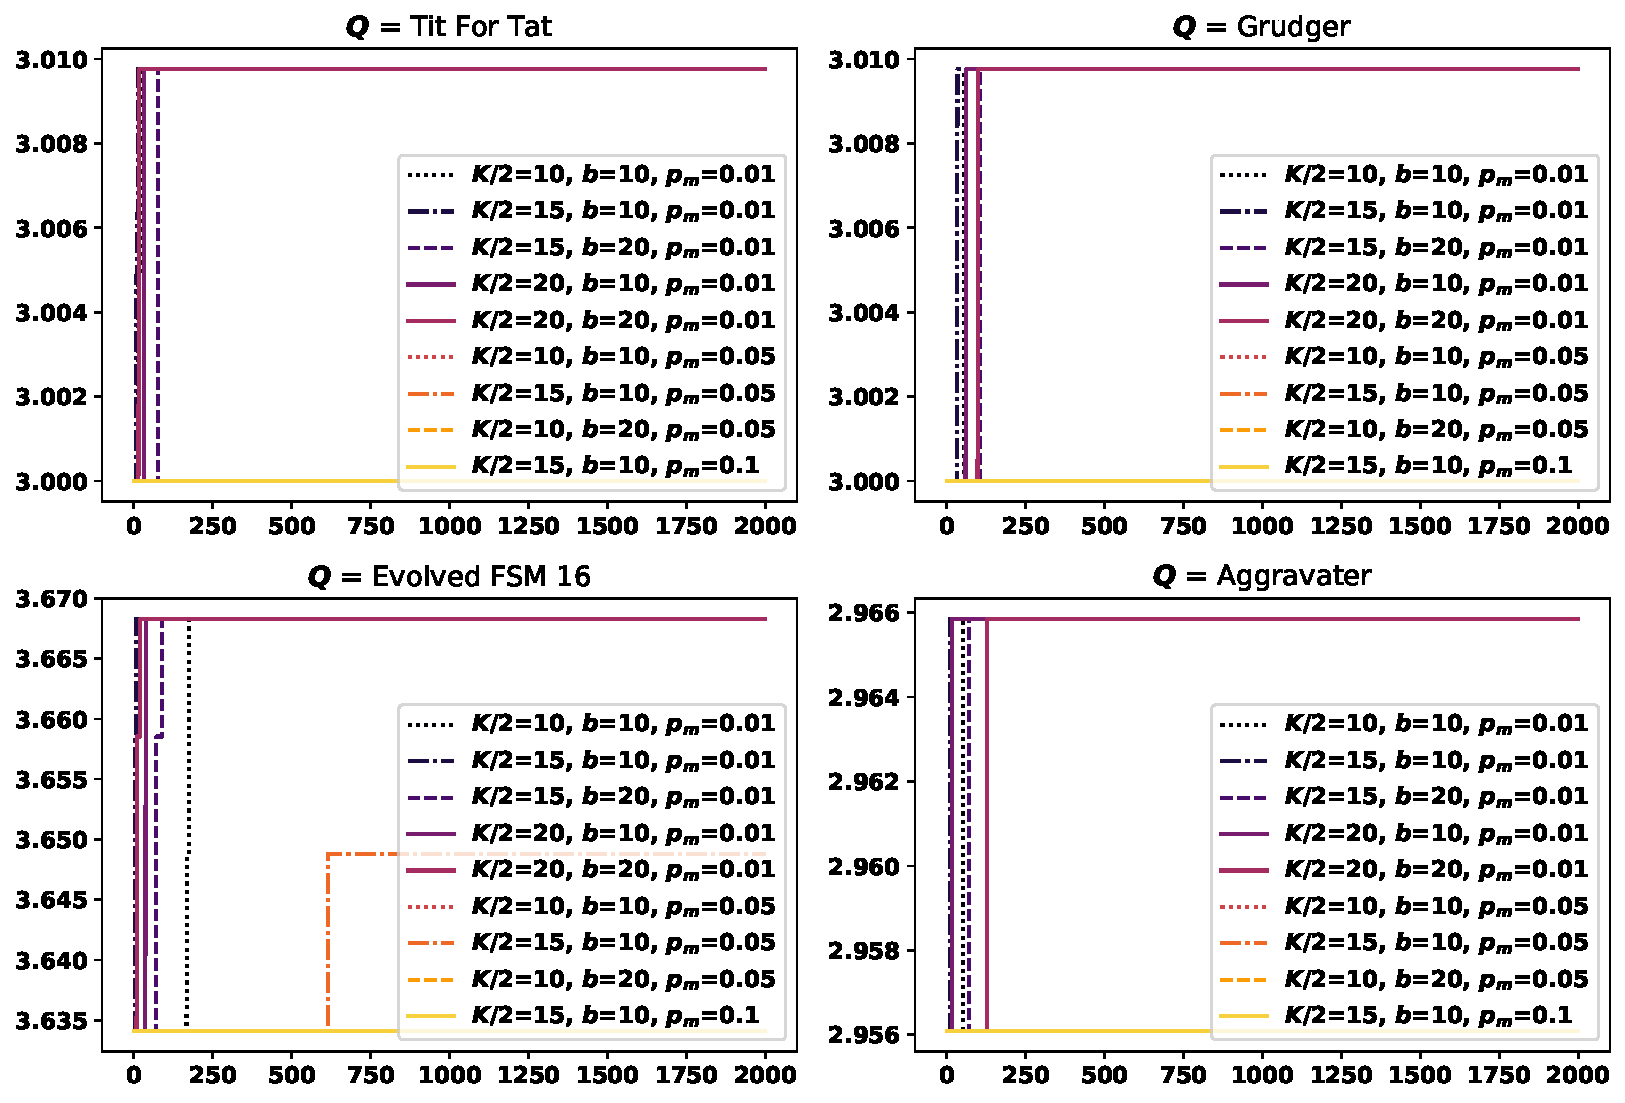
\includegraphics[width=.9\textwidth]{src/chapters/06/img/gas_results_per_trial.pdf}
    \caption{The highest score in a population over the generations for Tit For Tat,
    Grudger, FSM 16 and Aggravater. The selected trials capture the results
    of all the 18 trials for the given set of opponents.}\label{fig:ga_trials}
\end{figure}

Nevertheless, a sequence that has not converged is still useful. Even though
it is not the highest scoring member, it is a sequence that was not arbitrarily
generated but has some critical information regarding playing against given
opponents.

There are several trials that have managed to reach convergence,
and they did so in less than 200 generations. This is potentially the effect of a
non random initial population.
Figure~\ref{fig:ga_trials_to_500}
shows the highest score in a population over the generations for the four
strategies of Figure~\ref{fig:ga_trials} but only up to \(g_i = 500\). All trials
with a \(p_m=0.01\) reach convergence within the first 200 generations. The trial
which reaches convergence first (in the four demonstrated cases) is the trial
with the parameter values of \(K/2=15, b=10\) and \(p_m=0.1\).

\begin{figure}[!htbp]
    \centering
    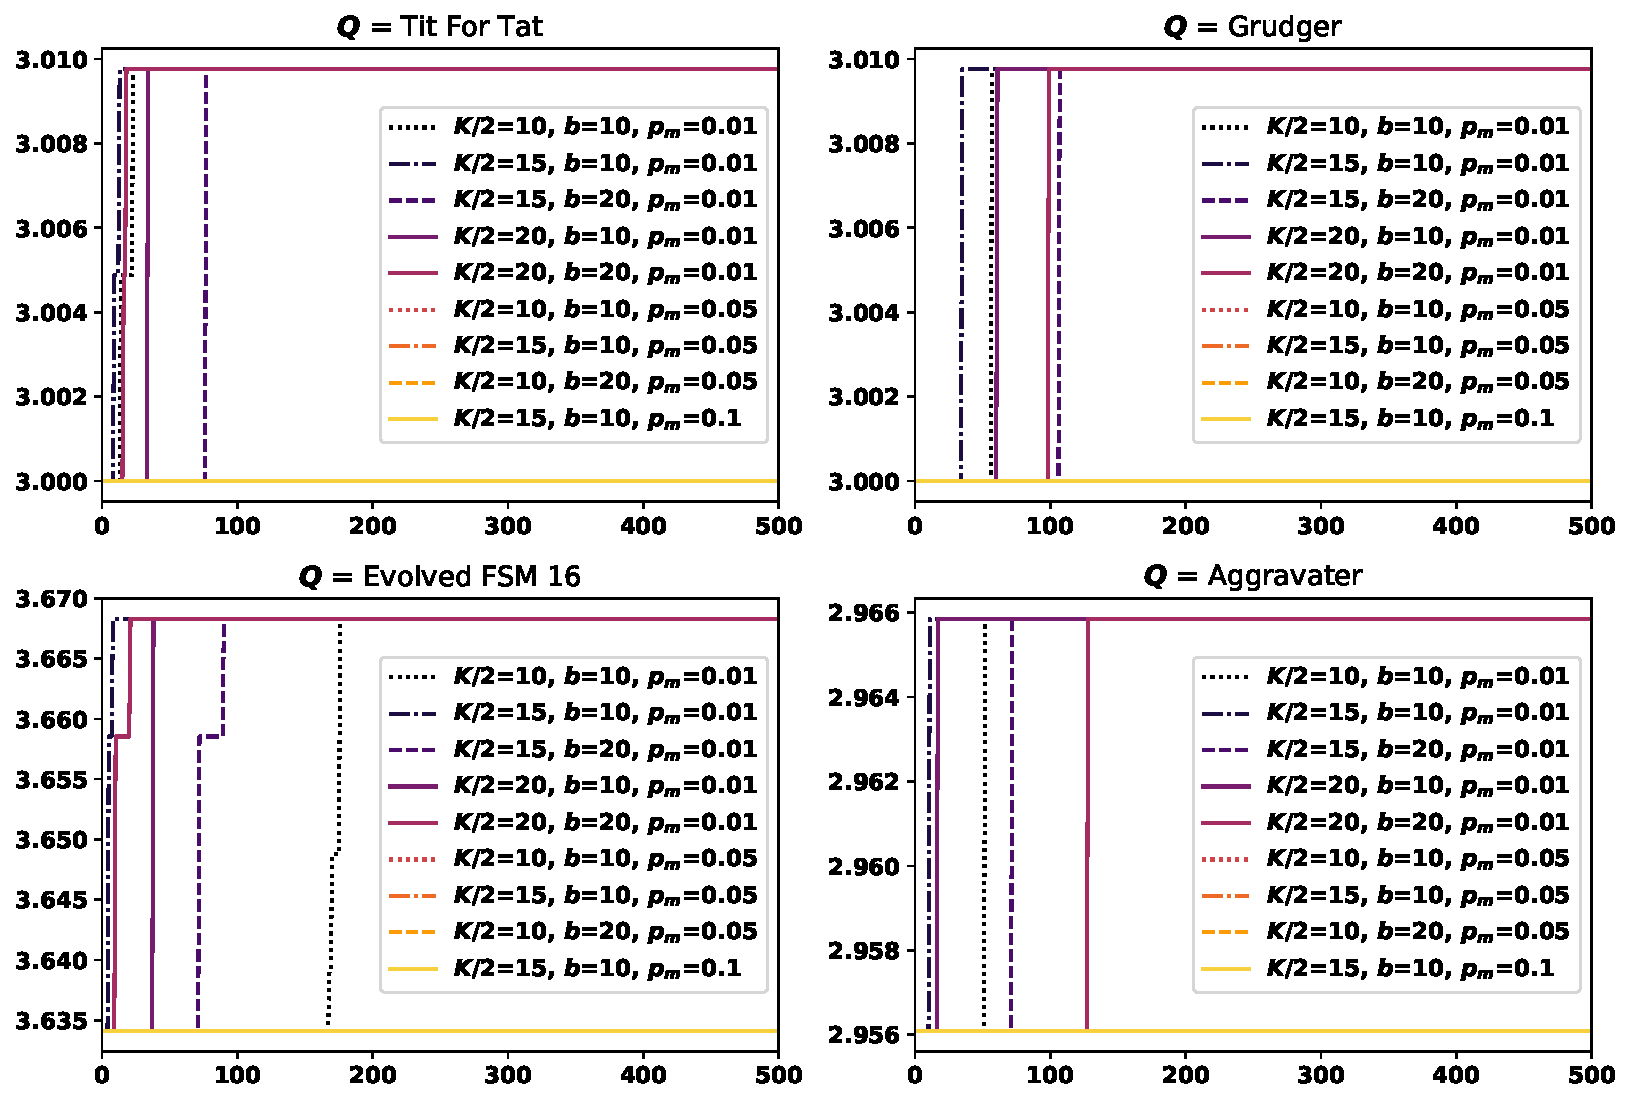
\includegraphics[width=.9\textwidth]{src/chapters/06/img/gas_results_per_trial_to_generation_500.pdf}
    \caption{The highest score in a population over the generations for Tit For Tat,
    Grudger, FSM 16 and Aggravater up to \(g_i = 500\).}\label{fig:ga_trials_to_500}
\end{figure}

There are a total of \deterministicstrategies deterministic strategies in the
collection of opponents and best response sequences were estimated for each.
Several of the known best response sequences have been manually checked and they
have been successfully estimated by the algorithm. These include best response
sequences to Tit For Tat, Grudger, Alternator, Pavlov and the Cycler strategies.

In section~\ref{section:ipd_as_sequences} is was explained that strategies can
have more than a single best response sequence. In the case of the strategy
Adaptive any strategy that cooperated twice in the opening 6 moves and defected
thereafter is a best response. The data collection has managed to successfully identify
multiple best responses to Adaptive, these are given by
Table~\ref{table:adaptive_best_responses}. Adaptive is not the only
deterministic strategy with multiple best response sequences. More specifically,
for the \deterministicstrategies deterministic opponents a total of \deterministicsequences best
response sequences were collected.

\begin{table}[!htbp]
    \resizebox{\textwidth}{!}{
    \begin{tabular}{lrrrrrrrrrrr}
\toprule
index &  gene 0 &  gene 1 &  gene 2 &  gene 3 &  gene 4 &  gene 5 &  gene 6 &  \(\dots\) &   gene 202 &  gene 203 &  gene 204 \\
\midrule
0     &       1 &       0 &       0 &       0 &       0 &       1 &       0 &  \(\dots\) &         0 &         0 &         0 \\
1     &       0 &       0 &       1 &       1 &       0 &       0 &       0 &  \(\dots\) &         0 &         0 &         0 \\
2     &       1 &       1 &       0 &       0 &       0 &       0 &       0 &  \(\dots\) &         0 &         0 &         0 \\
\bottomrule
\end{tabular}
}
    \caption{Best responses sequences estimated by the data collection process.
    Note that \(0\) corresponds to defection and \(1\) to cooperation.}
    \label{table:adaptive_best_responses}
\end{table}

An interesting questions that arises is: how diverse are the set of best response
sequences? Out of the \deterministicsequences sequences \stochasticuniquesequences are unique. A graphical
representation of these sequences is given by Figure~\ref{fig:brs_visualisation}.
The two distinct colours represent genes of \(C\) and \(D\). Overall, it can be
seen that there is diversity in the best response sequences, and they are not just
long sequences of either \(C\) or \(D\). A common trend appears to be a series
of defections at the last turns. In a finite IPD this is to expected. As it was
mentioned in Chapter~\ref{chapter:meta_tournaments}, as the likelihood of a
match ending in the following turn increases the effectiveness of defecting.

A total of \stochasticsequences sequences have been estimated for the stochastic opponents. From
these sequences, \reproducible did indeed play against the correct seeded opponent and
achieved their respective scores at the final generation.

For instance for the strategy - seed combination of Champion - seed\(=9\) the highest score
achieved by a member of the population over the generations is given by
Figure~\ref{fig:champion_ga_score}. There is variation in the highest score
occurring over the generations with several increasing and decreasing peeks. However,
for most of the generations the highest score appears to be between \(3.80 - 3.82\).
The best response sequence retrieved by the data collection scored 3.82 against
Champion, and it reflected the score of the sequence against Champion - seed\(=9\).

\begin{figure}[!htbp]
    \centering
    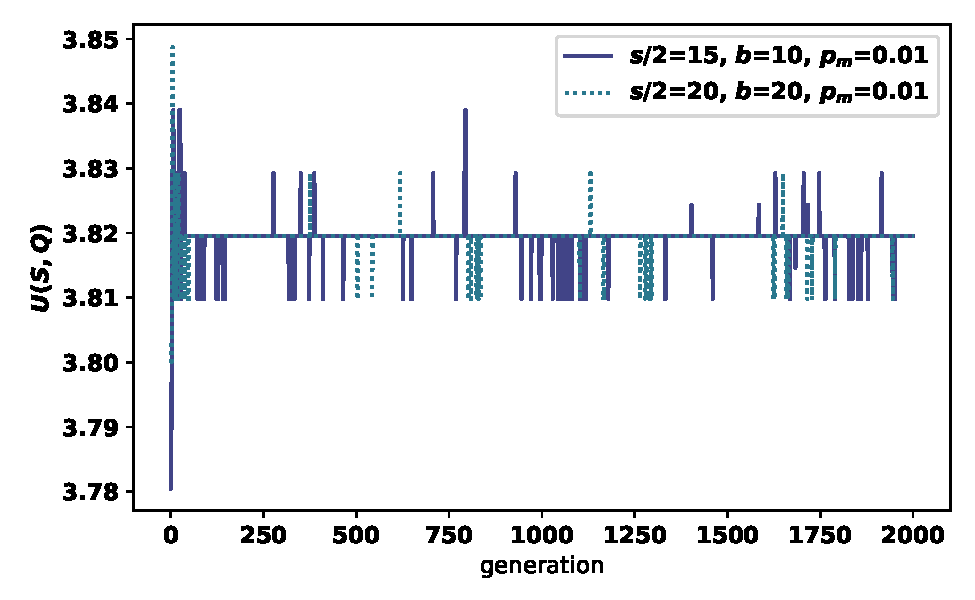
\includegraphics[width=.7\textwidth]{src/chapters/06/img/maximum_score_per_generation_champion.pdf}
    \caption{The maximum score a sequence achieved against Champion with seed 9
    over the generations. Each line represents a different GA trial. Only the
    GAs with \(p_m=0.01\) have been included.}\label{fig:champion_ga_score}
\end{figure}

There are stochastic opponents for which more variation occurred over the
generations. An example of that is Random. The highest score
of the population in a single GA trial, for opponent - seed combination Random -
seed\(=1\), is given by Figure~\ref{fig:random_ga_score}.
In the case of Random - seed\(=1\) the score of the best response sequence that
was collected was not the actual score the sequence scores against Random -
seed\(=1\).

\begin{figure}[!htbp]
    \centering
    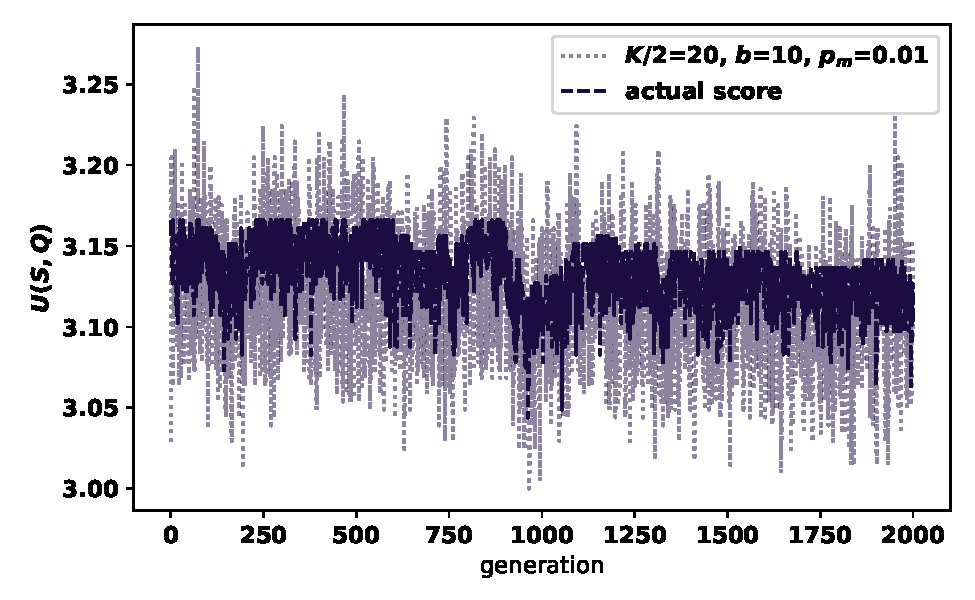
\includegraphics[width=.7\textwidth]{src/chapters/06/img/maximum_score_per_generation_random.pdf}
    \caption{The maximum score a sequence achieved against Random - seed\(=1\)
    over the generations.}\label{fig:random_ga_score}
\end{figure}

From the \stochasticsequences sequences against stochastic strategies \stochasticuniquesequences are unique. A graphical representation of 1000 of
those sequences are given by Figure~\ref{fig:brs_visualisation_stochastic}.
Similar to the results of the best response sequences against deterministic
opponents the sequences are diverse.

\begin{figure}[!htbp]
    \begin{subfigure}{0.45\textwidth}
    \centering
    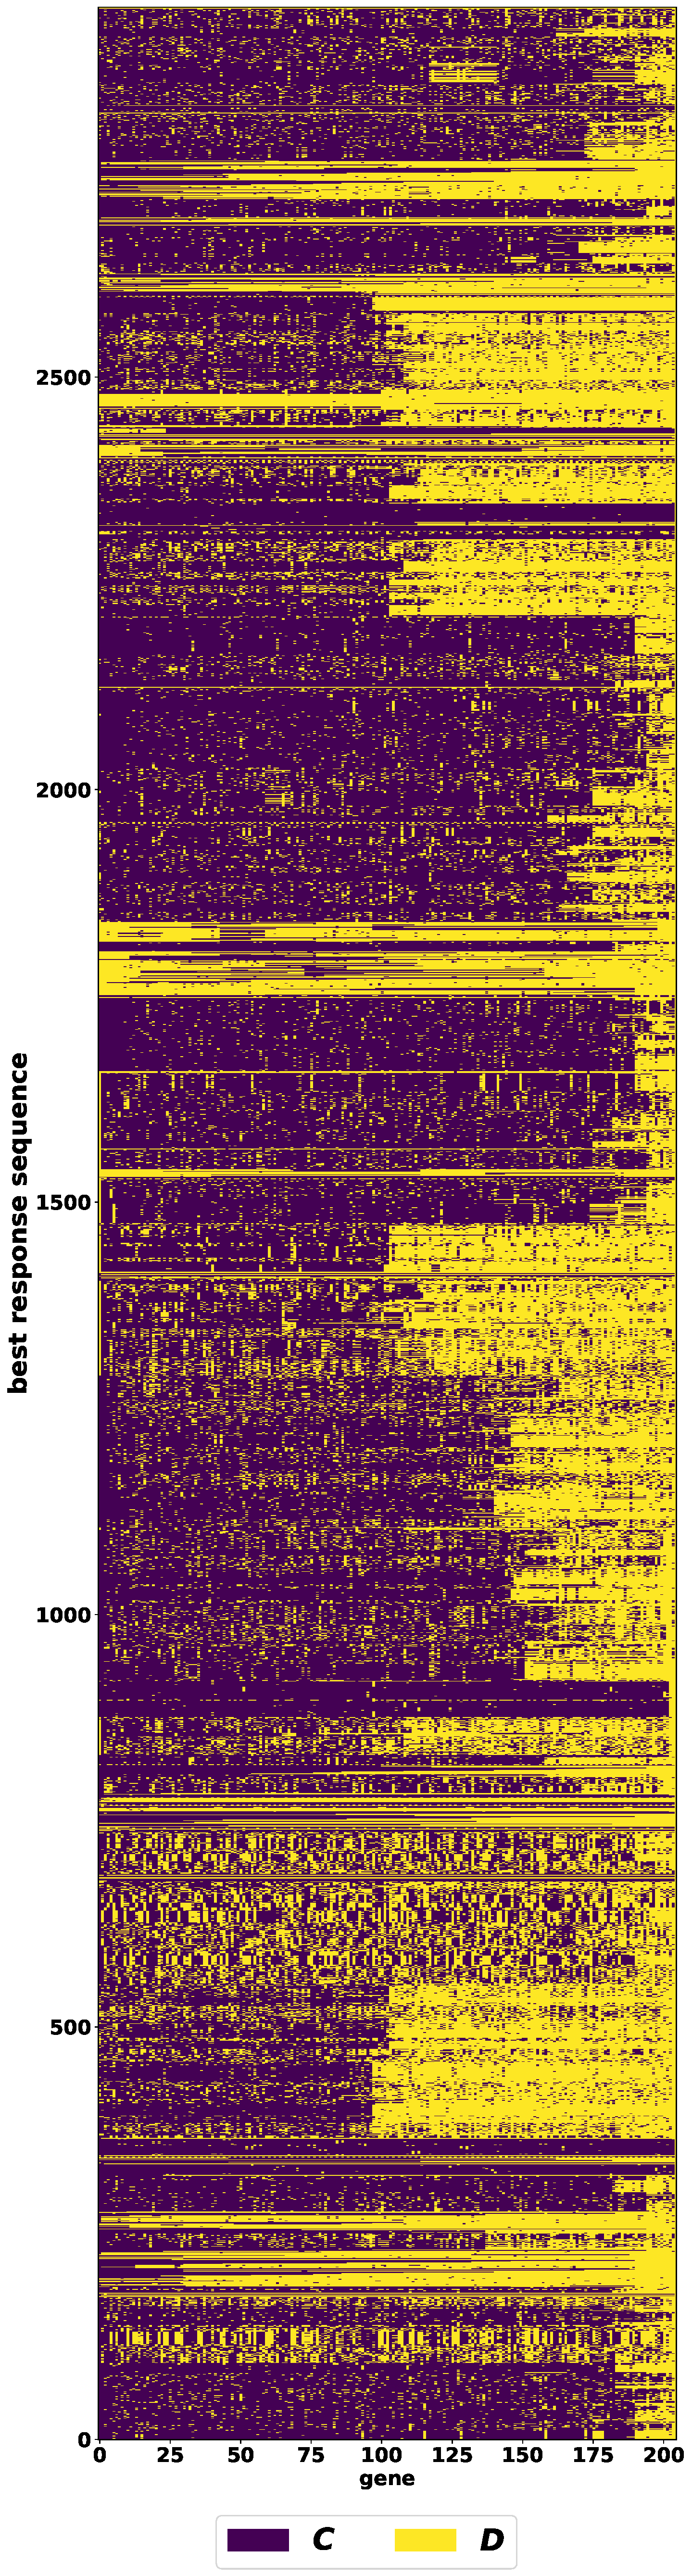
\includegraphics[width=\textwidth]{src/chapters/06/img/deterministic_best_responses.pdf}
    \caption{A graphical representation of best \deterministicsequences response sequence. These
    have been estimated using deterministic opponents.}\label{fig:brs_visualisation}
    \end{subfigure}\hfill
    \begin{subfigure}{0.45\textwidth}
    \centering
    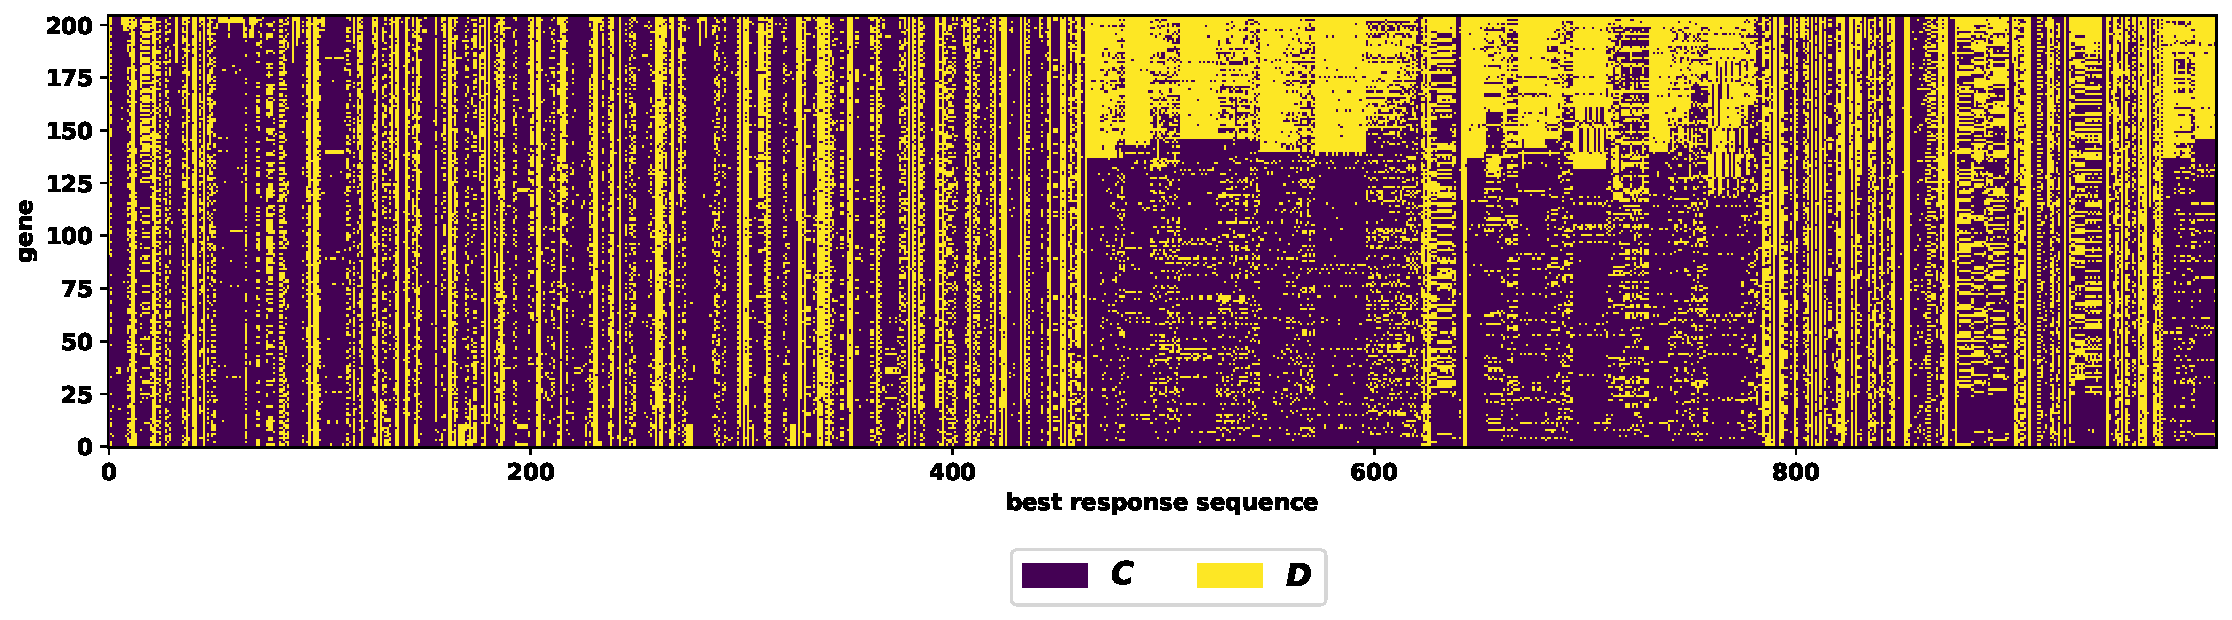
\includegraphics[width=\textwidth]{src/chapters/06/img/stochastic_best_responses.pdf}
    \caption{A graphical representation of \stochasticsequences response sequence. These
    have been estimated using stochastic opponents.}\label{fig:brs_visualisation_stochastic}
    \end{subfigure}
\end{figure}

In summary, from the list of \numberofstrategiesbestsequences strategies
examined in this Chapter, 750 different opponent instances were simulated and a
total of \totalsequences best response sequences of length 205 were retrieved. The choice of
205 turns will be explained in the following Chapter. The best response sequences have
been archived and made available at~\cite{Glynatsi2020_sequences}.

\section{Chapter Summary}

This Chapter has explored the concept of best responses in the IPD game in the
form of static sequences of moves. It introduced an evolutionary algorithm,
Algorithm~\ref{algorithm:genetic_algorithm}, which can successfully identify
best response sequences.

The algorithm was executed to estimate best response sequences to the majority
of opponents listed in the APL. More specifically, a total of
\numberofstrategiesbestsequences opponents from APL were used. Several of the
strategies in the project are stochastic and computer seeded versions of these
strategies were used to explore their different behaviours. From the list of
\numberofstrategiesbestsequences opponents a total of 750 different behaviours
were simulated.

For the \deterministicstrategies deterministic strategies a total of \deterministicsequences
sequences, from which \deterministicuniquesequences were unique, were estimated. These sequences were not
just a set of trivial sequences of either \(C\) or \(D\). A common trait in the
best response sequences appeared to be a series of defection closer to the final
turns. For the seeded versions of the \stochasticstrategies stochastic opponents
the best response sequences are not guaranteed to have been captured due to issues related to PRNGs and multi threading.
Nevertheless, a total of \stochasticsequences sequences from which \stochasticuniquesequences are unique were
collected. Similar, these sequences are more diverse than just a series of
a single action. The \totalsequences sequences that were collected have been
archived and are available at \cite{Glynatsi2020_sequences}.

The main purpose of this Chapter has been to generate the bespoke data set,
which contains a large number of unique and diverse sequences,
so it can be used as training data set for Chapter~\ref{chapter:lstm}.
